% $Id: conclusion.tex 
% !TEX root = main.tex

%%
\section{Adaptive \ac{RL} Agents with Changing Behavior}
\label{sec:implementation}

This section introduces \adaptiverl, our proposed approach for enabling \ac{RL} agents to dynamically adapt their behavior in response to evolving environmental conditions. Our method allows agents to pursue varying objectives throughout their operational lifespan and acquire new capabilities as tasks change over time. The implementation is publicly available\footnote{Available at: \url{https://github.com/rulas99/rl_uniandes}}.

The conceptual foundation of \adaptiverl aligns with the ideas proposed by~\citet{abel2023definitioncontinualreinforcementlearning}, emphasizing continual adaptation rather than convergence to a fixed solution. We extend tabular Q-learning by integrating adaptive mechanisms that enable agents to dynamically adjust their learning strategies in response to detected environmental changes. Similar to the approach described by~\citet{norman2024firstexploreexploitmetalearningsolve}, our agent thoroughly explores the environment each time a change is detected, subsequently exploiting the acquired knowledge. This strategy facilitates rapid convergence to new environment configurations without entirely discarding previously learned knowledge.

To enable dynamic behavioral adaptation, we introduce adaptive mechanisms that adjust the agent’s learning rate and exploration rate in conjunction with a concept drift detection strategy. By continuously monitoring and responding to changes in the environment, our agent can autonomously modify its learning process at runtime to maintain effective goal pursuit. This capability positions our approach within the class of self-adaptive systems (SAS), as defined by~\citet{sasreview}, ensuring continual adaptation and resilience in non-stationary contexts.

We dynamically adjust the learning rate based on the Temporal Difference (TD) error, as defined in~\eqref{eq:td_error}.

\begin{equation}
    \label{eq:td_error}
    TD_{error} = r_{t+1} + \gamma \cdot \underset{a}{\max} Q(s_{t+1}, a) - Q(s_t, a_t)
\end{equation}

This error quantifies the difference between the agent’s predicted reward and the actual reward received. The dynamic learning rate ($\alpha^*$) is then adjusted based on the TD error, as defined in~\eqref{eq:dynamic_learning_rate}.

\begin{equation}
    \label{eq:dynamic_learning_rate}
    \alpha^* = \alpha + (\alpha_{\max}-\alpha) \cdot \frac{1}{1 + e^{-(|TD_{error}|-k)}}
\end{equation}

In this formulation, $\alpha$ denotes the base learning rate (e.g., 0.1), while $\alpha_{\max}$ specifies its upper bound (e.g., 0.99). The parameter $k$ controls the sensitivity of the learning rate to the TD error, with higher values resulting in reduced sensitivity; thus, $k$ must be carefully tuned according to the specific characteristics of the environment and learning context. High TD errors induce a larger learning rate, enabling faster updates during exploration, whereas lower TD errors yield a more stable and conservative learning process during exploitation phases. In Figure~\ref{fig:alpha}, we illustrate the behavior of the dynamic learning rate ($\alpha^*$) in our Non-Stationary GridWorld experiments~\ref{sec:experiments}.

\begin{figure*}
    \centering
    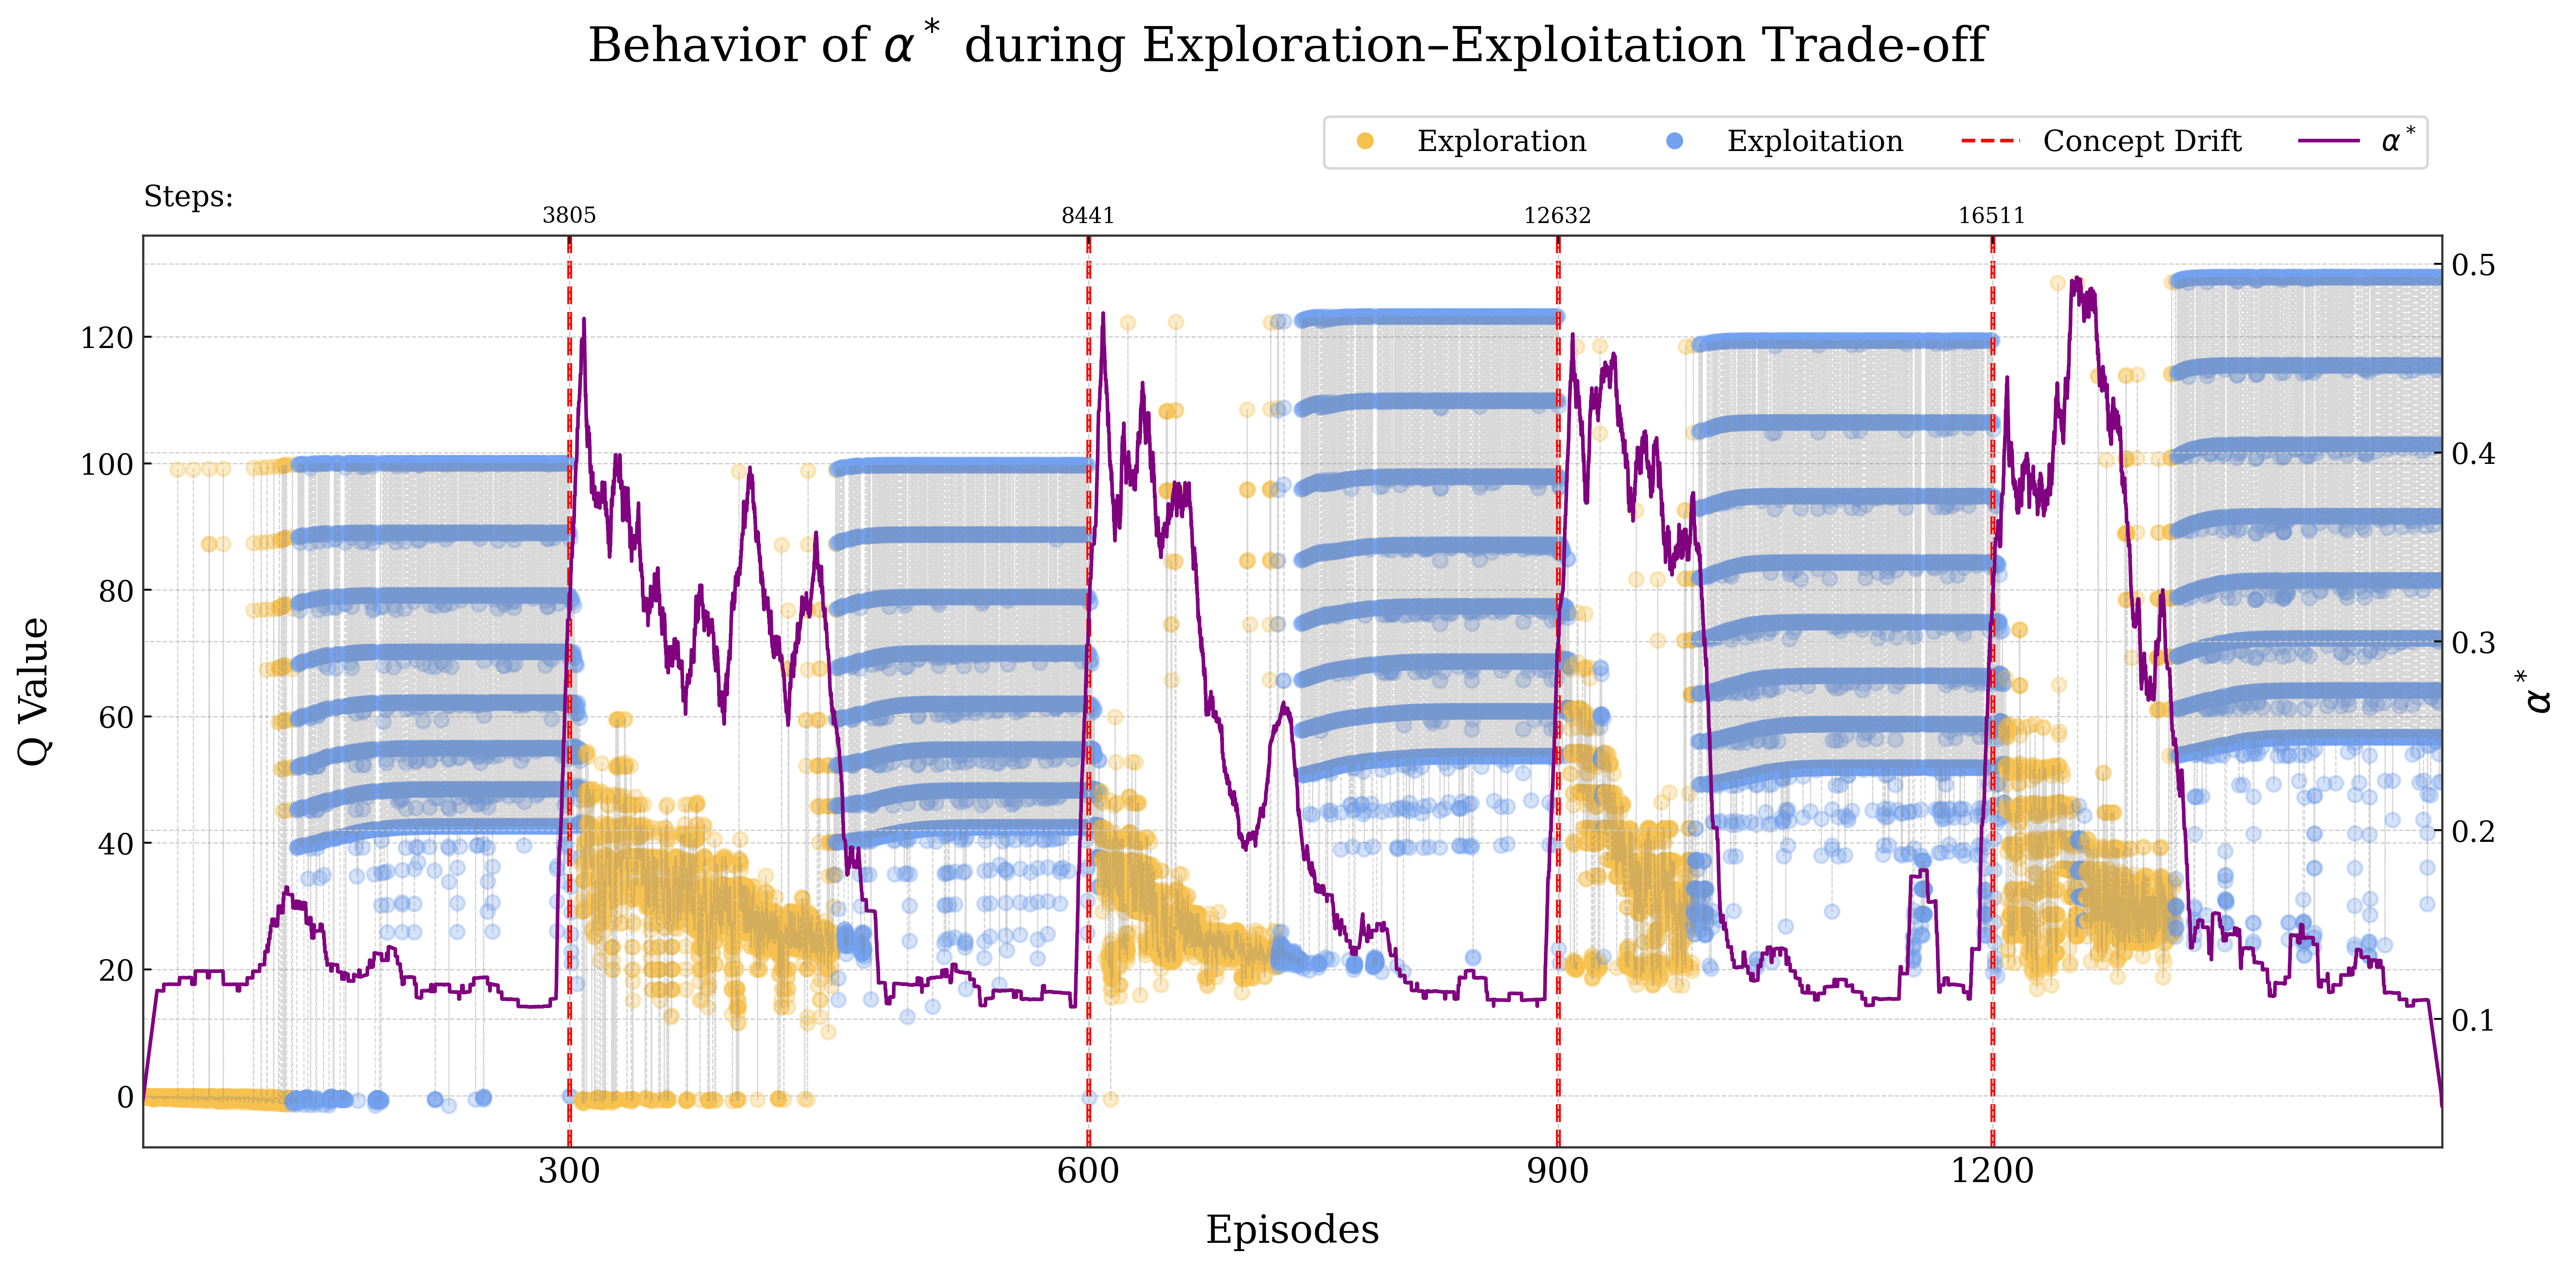
\includegraphics[width=\textwidth]{figures/alpha.png}
    \caption{Behavior of dynamic learning rate ($\alpha^*$) over Non-Stationary GridWorld experiments. Notice how $\alpha^*$ increases when the agent is exploring $\rightarrow$ high TD error and decreases when the agent is exploiting (low TD error), achieving a fast convergence during exploration and a stable learning during exploitation.}
    \label{fig:alpha}
\end{figure*}

Following the methodologies of~\citet{mignon2017adaptive} and~\citet{networkdynamicrl}, we implement the PH-test to detect significant shifts in the reward distribution at the end of each episode. The PH-test calculates a cumulative difference between observed rewards and the running mean reward, incorporating a sensitivity parameter ($\delta$). A concept drift (environmental change) is flagged when this cumulative difference surpasses a predefined threshold. Selecting an appropriate threshold value is crucial, as it determines the sensitivity of drift detection. Higher thresholds result in more conservative detection, while lower thresholds increase sensitivity to changes, this value must be selected based on the magnitude order of rewards and posible changes over them.

Building on the concept drift detection mechanism and inspired by~\citet{mignon2017adaptive}, we adaptively increase the exploration rate ($\varepsilon$) whenever the PH-test detects a concept drift. This approach promotes exploration immediately following environmental changes, enabling the agent to acquire new knowledge by temporarily adopting an exploration-focused policy. To ensure adequate exploration, the agent maintains this elevated exploration rate for a period (until rewards stabilize, i.e., no further drifts are detected) before $\varepsilon$ resumes its usual decay toward a minimal value, thereby returning to the exploitation phase.

This adaptive exploration mechanism ensures the agent maintains an effective balance between exploring new environment dynamics and leveraging previously acquired knowledge. It is crucial to sustain high exploration levels after consistent concept drift detection, so the agent can learn new policies without forgetting previously learned ones. In Figure~\ref{fig:dynamic-eps}, we illustrate the behavior of the dynamic exploration rate ($\varepsilon^*$) in our Non-Stationary GridWorld experiments~\ref{sec:experiments}.

\begin{figure*}
    \centering
    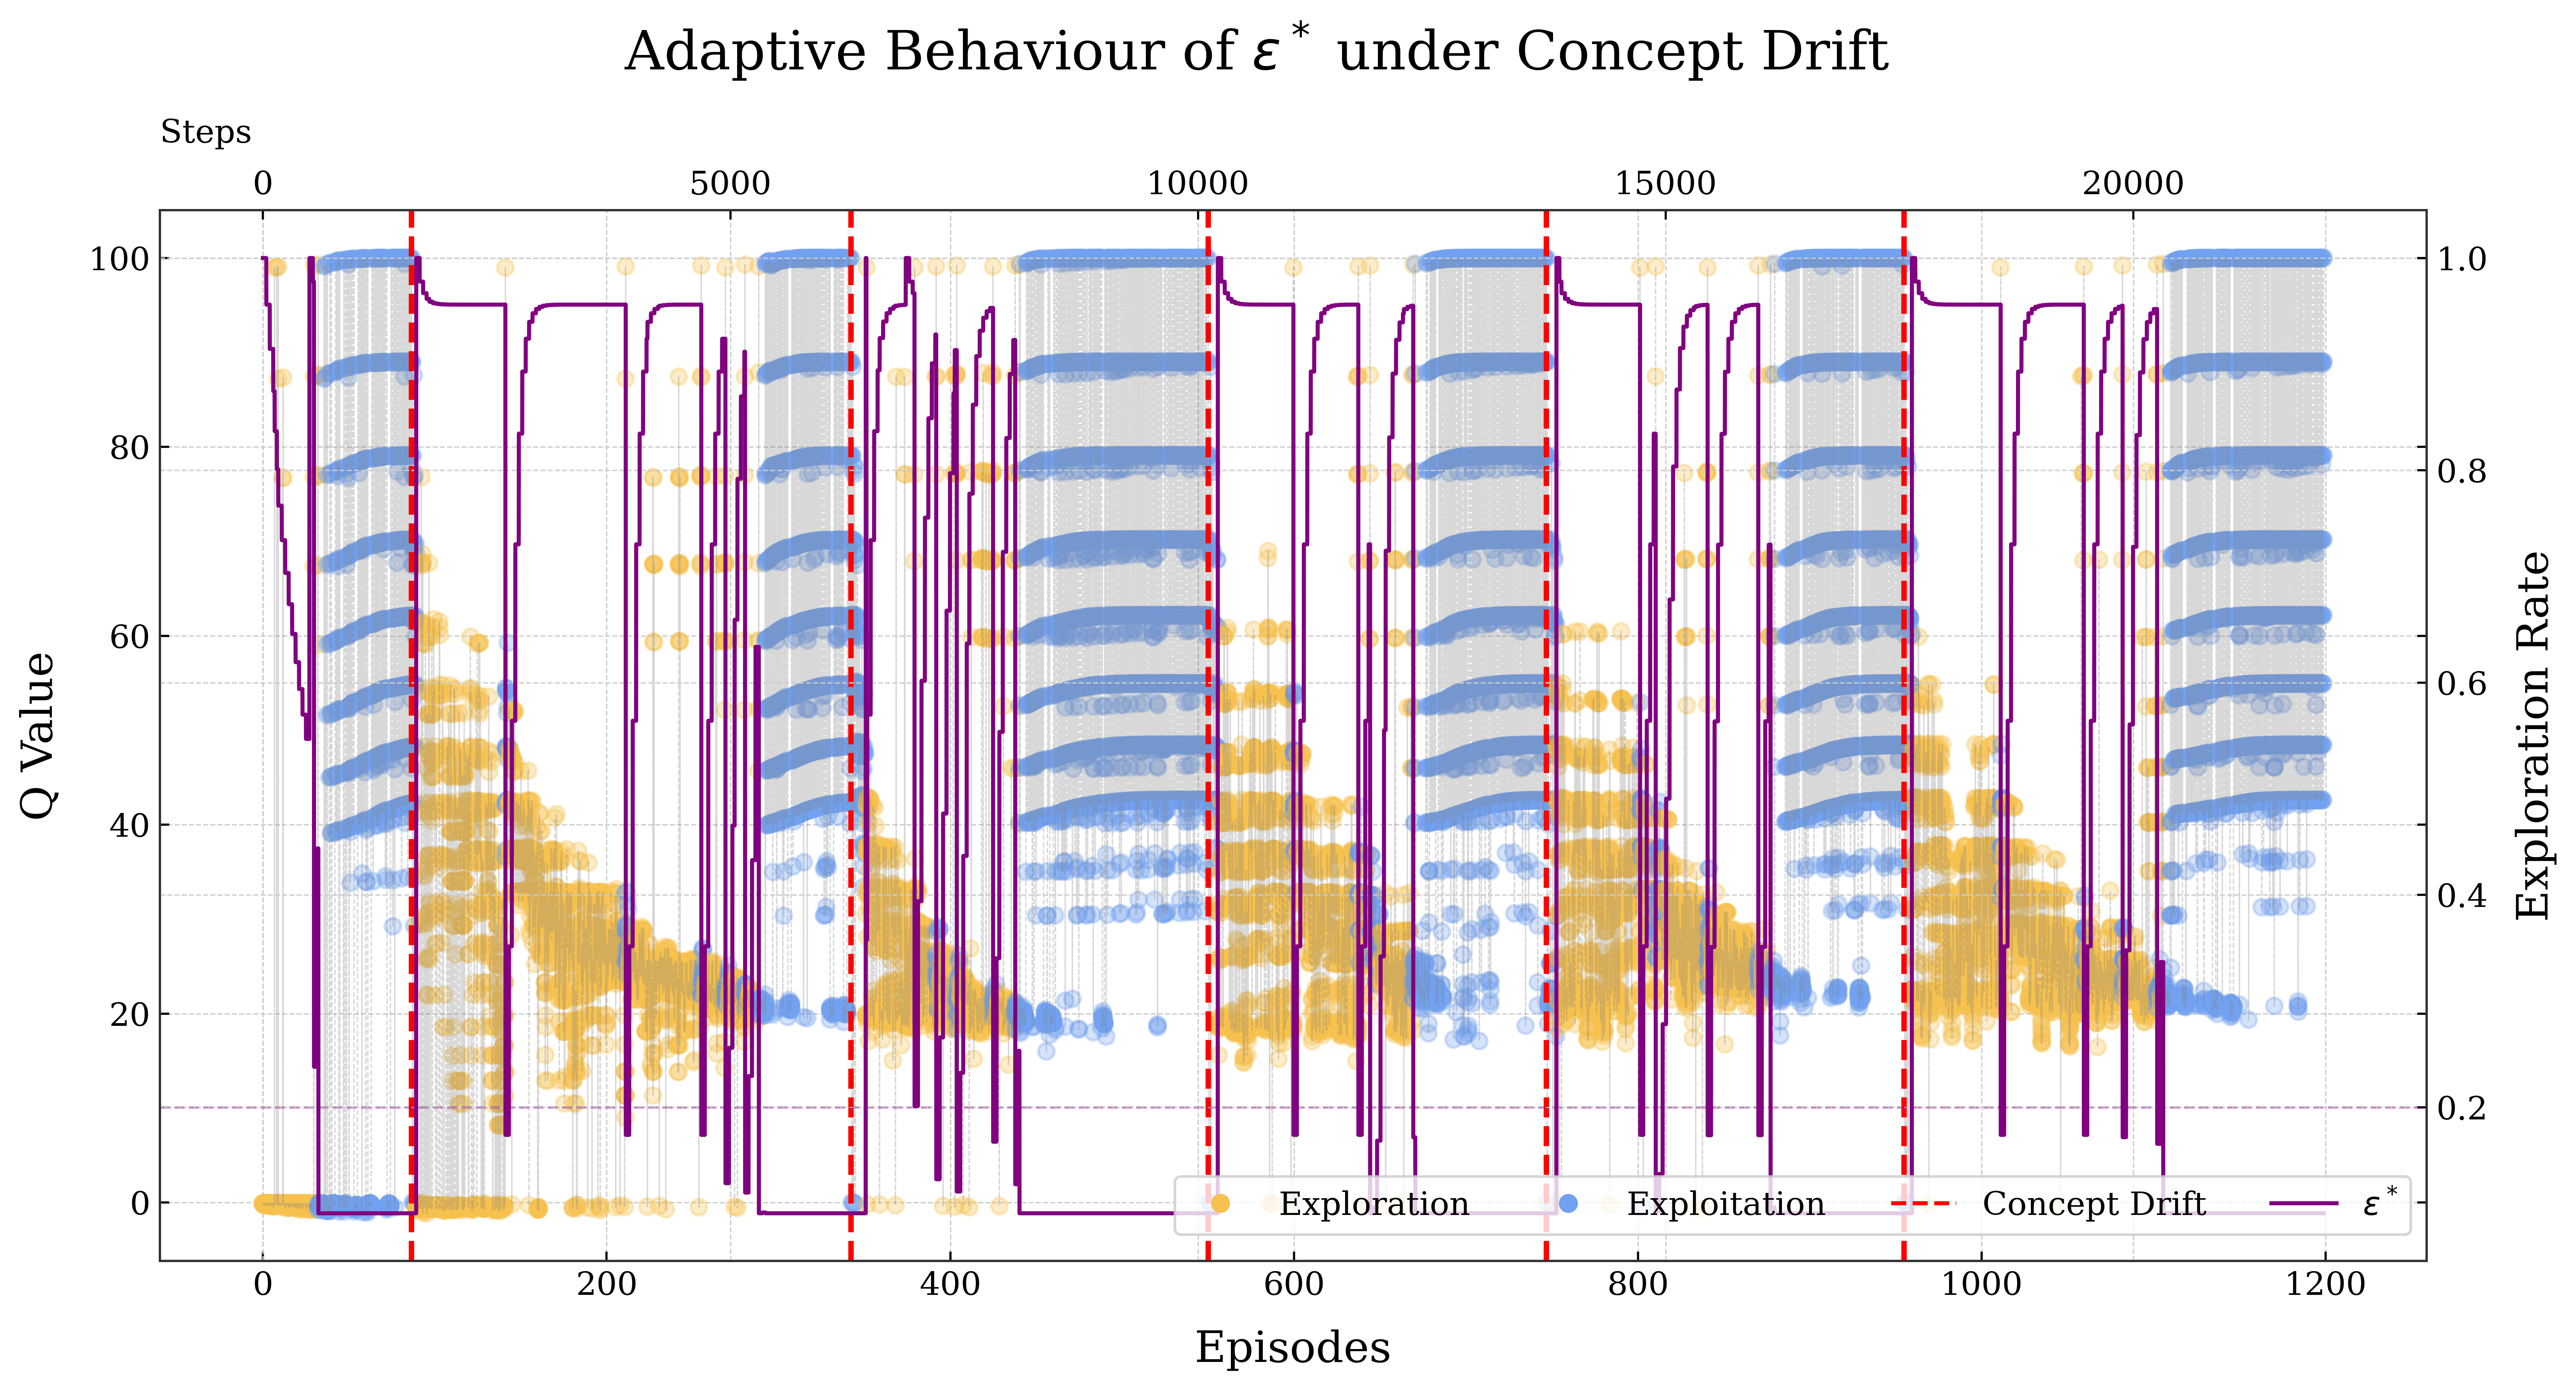
\includegraphics[width=\textwidth]{figures/epsilon.png}
    \caption{Behavior of the dynamic exploration rate ($\varepsilon^*$) in Non-Stationary GridWorld experiments. Notice how $\varepsilon^*$ increases each time a concept drift is detected by the PH-test and remains high until the agent consistently achieves the expected rewards (i.e., no further concept drift and stable rewards). Afterward, $\varepsilon^*$ begins to decay toward its minimum value allowing to explode the acquired knowledge.}
    \label{fig:dynamic-eps}
\end{figure*}

These adaptive mechanisms equip the agent to effectively manage learning under varying and unpredictable conditions, enabling continuous adaptation and efficient knowledge transfer between different environmental states. This approach allows the agent to rapidly respond to new information without discarding previously learned knowledge, achieving greater resilience and performance stability over its lifespan. In continous, we present a GridWorld example to illustrate \adaptiverl's behavior in am environment with non-stationary reward function and compare it with a standard Q-learning agent.

%%%%
\subsection{Agent Adaptation to Different Goals}
\label{sec:experiments}

To evaluate \adaptiverl’s ability to adapt to environmental changes induced by a non-stationary reward function, and to compare its performance against traditional Q-learning, we construct a $9\times 9$ GridWorld. In this domain, every cell yields a reward of $-1$, except for a single goal state that provides $+100$. The agent begins each episode at the grid’s center and may move up, down, left, or right. Initially, the goal is placed in the top-left corner. After every 300 episodes—by which time the agent should have learned the optimal policy—we trigger a concept drift by relocating the goal to the diagonally opposite corner (bottom-right). We repeat this alternation for a total of 1,500 episodes, expecting the agent to detect each drift and re-converge to the new optimal policy. Figure~\ref{fig:r-change} illustrates this GridWorld setup and the reward relocations.

\begin{figure*}
    \centering
    \includegraphics[width=\textwidth]{figures/rewards_change.png}
    \caption{GridWorld environment with a non-stationary reward function: the agent starts at the center and aims for the goal, which alternates between the top-left and bottom-right corners every 300 episodes.}
    \label{fig:r-change}
\end{figure*}

We compare two agents over 1,000 independent runs:  
\begin{itemize}
  \item A \emph{standard Q-learning} agent, with fixed learning rate $\alpha=0.1$ and a fixed exponential decay for the exploration rate.
  \item An \emph{\adaptiverl} agent, employing the adaptive learning-rate and exploration-rate mechanisms described in above.
\end{itemize}
We measure (1) the number of episodes required to re-converge after each reward change, and (2) the total number of steps across all 1,500 episodes. Table~\ref{tab:multi} reports the mean and standard deviation of the steps-to-goal for each drift, as well as the overall steps.  

\begin{table}
    \centering
    \caption{Performance summary over 1,000 runs: average $\pm$ standard deviation of steps to reach the goal after each drift, and total steps for all 1,500 episodes.}
    \resizebox{\textwidth}{!}{
\begin{tabular}{l | c | c | c | c | c }
\toprule
\textbf{Agent} & \textbf{1st Change} & \textbf{2nd Change} & \textbf{3rd Change} & \textbf{4th Change} & \textbf{Total Steps} \\
\midrule
Q-Learning  & 256.40 $\pm$ 4.35\% & -- & -- & -- & 40,683.74 $\pm$ 1.33\% \\
\textbf{\adaptiverl} & 135.81 $\pm$ 9.31\% & 475.17 $\pm$ 5.80\% & 767.81 $\pm$ 3.13\% & 1,069.74 $\pm$ 2.45\% & 23,292.07 $\pm$ 6.33\% \\
\bottomrule
\end{tabular}
}

    \label{tab:multi}
\end{table}

\adaptiverl outperforms the standard Q-learning agent on every metric. Figures~\ref{fig:alpha} and~\ref{fig:dynamic-eps} show how \adaptiverl’s adaptive mechanisms enable rapid re-learning of the new goal location without erasing knowledge of previous configurations. This behavior addresses the challenge of overlapping or even contradictory subtasks, as discussed in~\cite{Bagus2022}, where identical state–action pairs may yield different rewards.

By contrast, the standard Q-learning agent converges reliably only to the first goal configuration. Figure~\ref{fig:static-eps} depicts its exploration rate decay: after each drift, the agent continues to exploit the old policy for an extended period, effectively “forgetting” previous knowledge before it begins learning the new goal location.

\begin{figure*}
    \centering
    \includegraphics[width=\textwidth]{figures/trad_eps.png}
    \caption{Behavior of the static exploration rate decay ($\varepsilon$) under traditional Q-learning: the agent fails to adapt to any subsequent goal relocation, exhibiting prolonged exploitation of the obsolete policy.}
    \label{fig:static-eps}
\end{figure*}


These results demonstrate that \adaptiverl consistently outperforms standard Q-learning in adapting to changing goals and acquiring new policies without forgetting previously learned knowledge. As shown in Figure~\ref{fig:q-value-comp}, after 1,500 episodes, \adaptiverl maintains high Q-values for all previous goal configurations, whereas traditional Q-learning must overwrite its Q-values each time the goal relocates. Notably, \adaptiverl preserves prior knowledge by promoting exploration for a sufficient period after each detected drift and by scaling updates according to the TD-error magnitude. This approach not only prevents catastrophic forgetting but also enables the agent to handle both contradictory and non-contradictory overlapping subtasks—such as when goals are randomly sampled in nearby regions rather than at the exact same cell\footnote{Animated simulations of these and other scenarios are available at: \url{https://github.com/rulas99/rl_uniandes/tree/main/simulations}}.

While \adaptiverl introduces modest overhead due to drift detection and adaptive updates, its overall runtime is actually lower: on an Intel Core i5 with 64 GB RAM, 1,000 runs require approximately 5 minutes for \adaptiverl, compared to 8 minutes for standard Q-learning. This efficiency gain results directly from the reduced number of steps needed to reach the goal after each drift. Specifically, \adaptiverl converges in significantly fewer steps than the standard agent—requiring about 1.9× fewer iterations after the first drift and 1.7× fewer over the full 1,500 episodes—highlighting the practical advantages of our adaptive mechanisms in dynamic environments.

\begin{figure*}
    \centering
    \includegraphics[width=\textwidth]{figures/q_map_comp.png}
    \caption{Comparison of Q-value heatmaps after 1,500 episodes: (left) \adaptiverl preserves high Q-values across alternating goal configurations; (right) traditional Q-learning must overwrite past knowledge to learn each new goal.}
    \label{fig:q-value-comp}
\end{figure*}

%%%%
\subsection{Agent acquisition of new capabilities}
In the next section~\ref{sec:validation}, we present a real-world use case for traffic light control, where the agent is provided with a new set of actions following concept drift detection. This enables the agent to efficiently learn how to utilize the new actions and optimize traffic flow by adapting its policy to varying congestion levels. The agent can acquire new capabilities without forgetting previously learned behaviors, maintaining adaptability to changing environmental conditions.

\endinput

